\chapter{Rotor-dynamic analysis}


\noindent
At this point, the tail-rotor behaviour has been investigated implementing a simplified FEM model and taking advantage of the Rotordynamics capabilities of Ansys. \\
Rotor-dynamics is the study of vibrational behaviour in axially symmetric rotating structures. At high rotational speeds, such as in a helicopter's tail rotor, the inertia effects of the rotating parts must be consistently represented in order to accurately predict the rotor behaviour. An important part of the inertia effects is the \underline{gyroscopic moment} introduced by the precession motion of the rotor which is function of the spin velocity. Hence, the velocity term in the equation of motion as well as the support flexibility and damping behaviour cannot be neglected and they are important factors in enhancing the stability of the vibrating rotor.



\section*{Modal analysis of rotating structures}
\addcontentsline{toc}{section}{Modal analysis of rotating structures}
\noindent
The modal analysis allows for the calculation of natural frequencies and critical speeds (Campbell diagram) of the rotor. \\
Dinamically speaking, the equations of motion of a generic rotating structure is:

\begin{equation*}
\left[ M \right] \left\lbrace \ddot{u} \right\rbrace + \left( \left[ C \right] + \left[ G \right] \right) \left\lbrace \dot{u} \right\rbrace + \left( \left[ K \right] - \left[ K_c \right] \right) \left\lbrace u \right\rbrace = \left\lbrace 0 \right\rbrace
\end{equation*}

\noindent
where [G] is the gyroscopic matrix that depends on the rotational velocity and is the major contributor to tailboom's rotor, while [$K_c$], the spin softnening matrix, also depends upon the rotational velocity and it modifies the apparent stiffness of the structure. \\
This equation holds when motion is described in a stationary reference frame.

\noindent
\underline{STEPS FOR MODAL ANALYSIS IN ANSYS}: \\
1) Model implementation; \
2) Boundary conditions; \
3) Solution includung rotational effects (centrifugal and Coriolis); \
4) Postprocessing.



\subsection*{Tail rotor simplified model}
\addcontentsline{toc}{subsection}{Tail rotor simplified model}
\noindent
A simplified model of the tail rotor has been defined, and it consists in the following parts:
\begin{itemize}
	\item \textbf{SHAFT}: elastically supported shaft modelled with BEAM 188 elements;
	\item \textbf{ROTOR'S HUB}: modelled with a lumped mass and inertia concentrated in the center of the rotor attached to a master node;
	\item \textbf{ROTOR}: modelled with a circular ring of SHELL 181 elements with radius passing through to the center of mass of the blades. CERIG elements have been introduced in order to connect the master node (hub) to the slave nodes of the ring.
\end{itemize}

\medskip
\begin{figure}[h]
	\begin{center}
		\centering  		 		
		\includegraphics[width=0.7\linewidth]{PICTURES/5_Rotordynamics/scheme.png}
	\end{center}
	\caption {Scheme of the simplified tail rotor model}
\end{figure}
%\vspace{0.5cm}

\medskip
\begin{figure}[h]
	\begin{center}
		\centering  		 		
		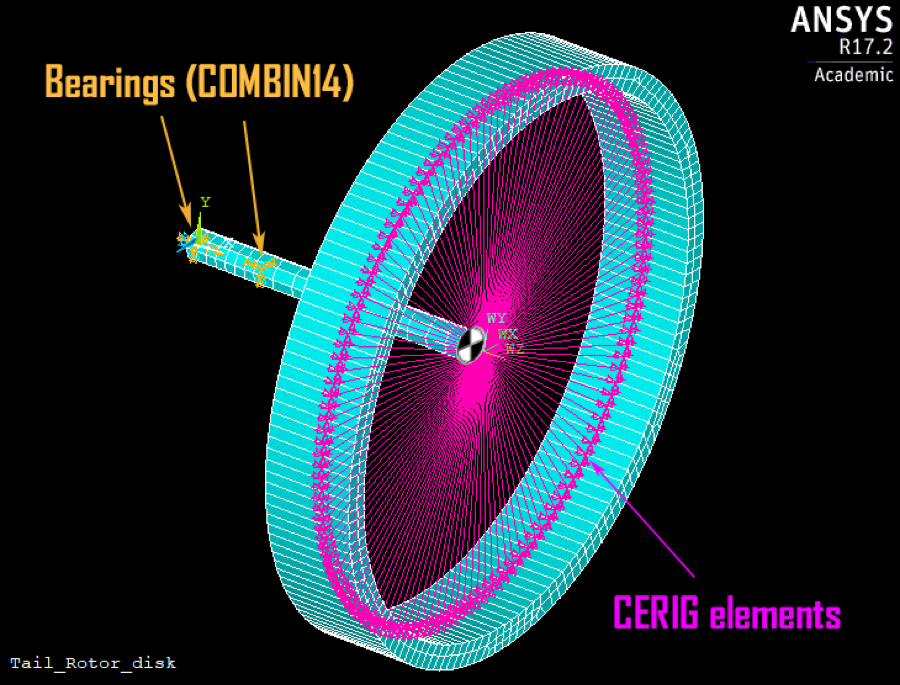
\includegraphics[width=0.9\linewidth]{PICTURES/5_Rotordynamics/2.png}
	\end{center}
	\caption {Tail rotor simplified model}
\end{figure}
%\vspace{0.5cm}

\subsection*{Model assumptions}
\addcontentsline{toc}{subsection}{Model assumptions}
\begin{itemize}
	\item Axial-symmetric structure (requirement for rotor-dynamics);
	\item Linear elastic material properties;
	\item Rotor elastically supported (2 bearings);
	\item Aerodynamic loads not considered;
	\item Rigid rotor and connections (no hinges or flexible joints).
\end{itemize}



\subsection*{Applied boundary conditions}
\addcontentsline{toc}{subsection}{Applied boundary conditions}
\noindent
\begin{itemize}
	\item Only fixed constraints are allowed for rotor-dynamic analysis;
	\item Support elasticity modelled using COMBIN14 elements to represent bearings;
\end{itemize}

\noindent
\textbf{COMBIN14} \\
Bearings have been modelled with COMBIN14 element whose properties simulate the effect of a longitudinal spring-damper as a uniaxial tension-compression element.
The element is created between two nodes which, in our case, are overlapped. One of the nodes is rigidly attached to the shaft while the other one is constrained on the ground. These elements allows the elastic movement of the shaft in the Y and Z directions. \\


\medskip
\begin{table}[h!]
	\centering
	
	\begin{tabular}{c c} 
		\toprule
		\multicolumn{2}{c}{Bearing's properties}\\
		\midrule
		Type & Stiffness K (N/m)  \\
		\midrule
		7 balls bearing & $378e+7$  \\ 
		\bottomrule
	\end{tabular}	
\end{table}
 

\clearpage
\subsection*{Solution including rotational effects (centrifugal and Coriolis)}
\addcontentsline{toc}{subsection}{Solution including rotational effects (centrifugal and Coriolis)}
\noindent
The modal analysis must be solved using an algorithm for damped modal analysis (complex Eigenvalues and Eigenvectors). We have chosen the \textbf{QRDAMP} solver including the rotational effects (\textbf{CORIOLIS, ON, , , ON}). \\ The rotation speed (2000 RPM) has been divided in several load-steps. 10 modes have been extracted from each step. \\

\lstinputlisting[firstline=133, lastline=146, language=apdl-modified]{./COMMAND_LISTS/SOLO_ROTOR.txt}



\subsection*{Postprocessing}
\addcontentsline{toc}{subsection}{Postprocessing}
\noindent
Rotor's natural frequencies have been calculated for each value of the rotation speed (hence for each load step) and assigned to a substep. Resulting natural frequencies vary with the rotor speed as it is displayed in the campbell diagram below. \\
A \textbf{critical speed} appears when the natural frequency is equal to the excitation frequency, and excitation may come from unbalance that is synchronous with the rotational velocity. \\
Critical speeds are directly determined by solving a new eigenvalue problem or by performing a Campbell diagram analysis, where the intersection points between the frequency curves and the excitation line are calculated.

\noindent
The rotational velocity of the rotor is specified via the \textbf{CMOMEGA} command which requires to specify which is the rotating component, previously defined and selected and to input the velocity vector (magnitude and direction). \\
Then, we can set the \textbf{CAMPBELL, ON} Ansys' command. \\

\noindent
\textbf{NOTE:} \\
Bearing stiffness has an important effect on the critical speeds. When analyzing a rotor, it is important to understand the effect of the bearing stiffness on the critical speeds and this can be done drawing the "Critical Speed Map" (here neglected).

\clearpage
\medskip
\begin{figure}[h]
	\begin{center}
		\centering  		 		
		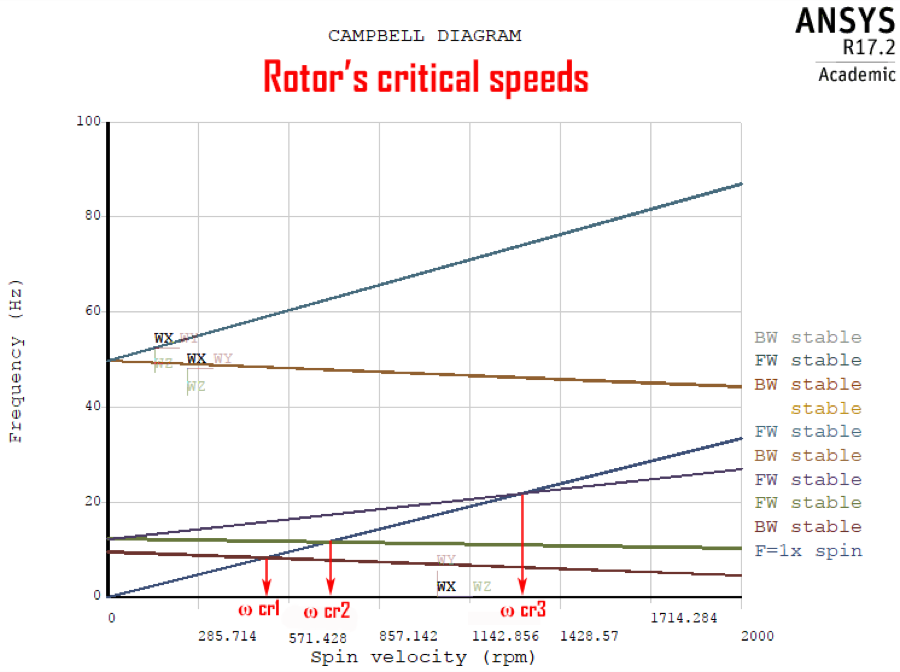
\includegraphics[width=0.95\linewidth]{PICTURES/5_Rotordynamics/campbell1.png}
	\end{center}

\end{figure}
%\vspace{0.5cm}







\begin{table}[h!]
	\centering
	\pgfplotstableset{
		% global config, for example in the preamble
		% these columns/<colname>/.style={<options>} things define a style
		% which applies to <colname> only.
		every head row/.style={before row=\hline,after row=\hline},
		every last row/.style={after row=\hline},
		display columns/0/.style={column name =Num, int detect,column type=r},
		display columns/1/.style={column name =Critical Speed [rpm], column type=r,
			fixed,fixed zerofill,precision=5,set thousands separator={\,}},
		%other style option   
	}
	\pgfplotstabletypeset[col sep=space]{VelocCritic-ModalAnalisys.txt}
	\caption{Natural frequencies for the simple model}
	\label{tab:ModalFreq-Shellmodel}
\end{table}


\clearpage
\smallskip
\begin{figure}[h!]
	\begin{center}
		\centering  		 		
		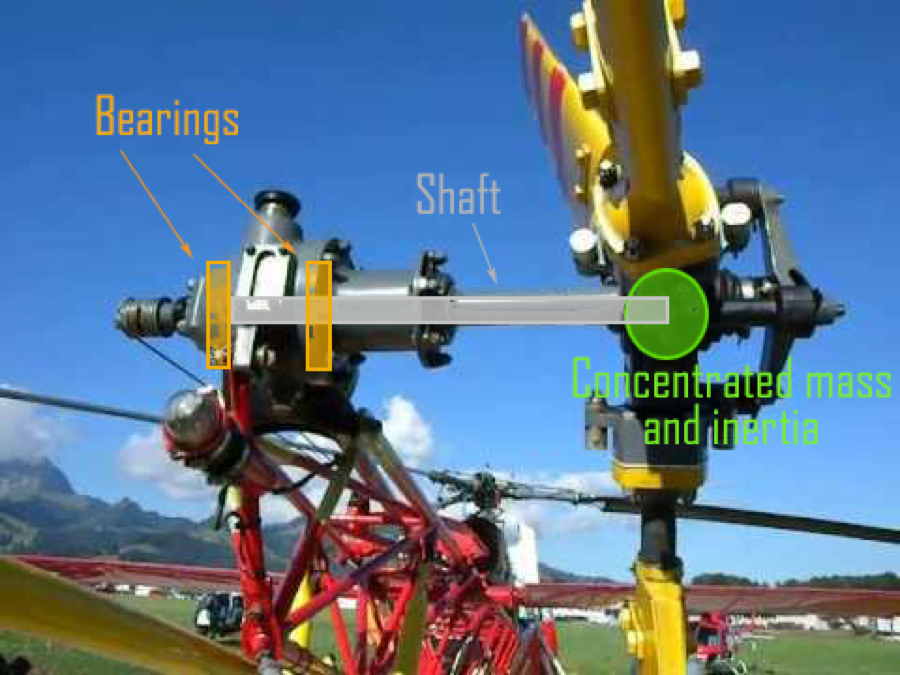
\includegraphics[width=0.9\linewidth]{PICTURES/2_Lama_truss/PNG/model2/hqdefault2}
	\end{center}
	\caption{Tail rotor assembly}
\end{figure}	
%\vspace{0.5cm}